%% abtex2-modelo-projeto-pesquisa.tex, v-1.7.1 laurocesar
%% Copyright 2012-2013 by abnTeX2 group at http://abntex2.googlecode.com/ 
%%
%% This work may be distributed and/or modified under the
%% conditions of the LaTeX Project Public License, either version 1.3
%% of this license or (at your option) any later version.
%% The latest version of this license is in
%%   http://www.latex-project.org/lppl.txt
%% and version 1.3 or later is part of all distributions of LaTeX
%% version 2005/12/01 or later.
%%
%% This work has the LPPL maintenance status `maintained'.
%% 
%% The Current Maintainer of this work is the abnTeX2 team, led
%% by Lauro César Araujo. Further information are available on 
%% http://abntex2.googlecode.com/
%%
%% This work consists of the files abntex2-modelo-projeto-pesquisa.tex
%% and abntex2-modelo-references.bib
%%

% ------------------------------------------------------------------------
% ------------------------------------------------------------------------
% abnTeX2: Modelo de Projeto de pesquisa em conformidade com 
% ABNT NBR 15287:2011 Informação e documentação - Projeto de pesquisa -
% Apresentação 
% ------------------------------------------------------------------------ 
% ------------------------------------------------------------------------

\documentclass[
	12pt,
	oneside,
	a4paper,
	english,
	brazil,
]{abntex2}

% ---
% PACOTES
% ---

% ---
% Pacotes fundamentais 
% ---
\usepackage{cmap}				% Mapear caracteres especiais no PDF
\usepackage{lmodern}			% Usa a fonte Latin Modern
\usepackage[T1]{fontenc}		% Selecao de codigos de fonte.
\usepackage[utf8]{inputenc}		% Codificacao do documento (conversão automática dos acentos)
\usepackage{indentfirst}		% Indenta o primeiro parágrafo de cada seção.
\usepackage{color}				% Controle das cores
\usepackage{graphicx}			% Inclusão de gráficos
\usepackage{xcolor}
\usepackage{tabularx}
% ---

% ---
% Pacotes de citações
% ---
\usepackage[brazilian,hyperpageref]{backref}	 % Paginas com as citações na bibl
\usepackage[alf]{abntex2cite}	% Citações padrão ABNT

% --- 
% CONFIGURAÇÕES DE PACOTES
% --- 

% ---
% Diretório das imagens
% ---
\graphicspath{ {Images/} }

% ---
% Configurações do pacote backref
% Usado sem a opção hyperpageref de backref
\renewcommand{\backrefpagesname}{Citado na(s) página(s):~}
% Texto padrão antes do número das páginas
\renewcommand{\backref}{}
% Define os textos da citação
\renewcommand*{\backrefalt}[4]{
	\ifcase #1 %
		Nenhuma citação no texto.%
	\or
		Citado na página #2.%
	\else
		Citado #1 vezes nas páginas #2.%
	\fi}%
% ---

% ---
% Informações de dados para CAPA e FOLHA DE ROSTO
% ---
\titulo{Aplicação que utiliza Beacons para automatizar a chamada em sala de aula}
\autor{Rafael Kellermann Streit}
\local{Brasil}
\data{2016}
\instituicao{%
  FACCAT - Faculdades Integradas de Taquara
  \par
  Graduação em Sistemas de Informação}
\tipotrabalho{Projeto de Pesquisa}
% O preambulo deve conter o tipo do trabalho, o objetivo, 
% o nome da instituição e a área de concentração 
\preambulo{Aplicação que faz a marcação de presença dos alunos em sala de aula de forma automatizada, utilizando Beacons.}
% ---

% ---
% Configurações de aparência do PDF final

% informações do PDF
\makeatletter
\hypersetup{
     	%pagebackref=true,
		pdftitle={\@title}, 
		pdfauthor={\@author},
    	pdfsubject={\imprimirpreambulo},
	    pdfcreator={LaTeX with abnTeX2},
		pdfkeywords={abnt}{latex}{abntex}{abntex2}{projeto de pesquisa}{beacon}{bluetooth}{ios}{mobile}, 
		colorlinks=false,       		% false: boxed links; true: colored links
    	linkcolor=black,          	% color of internal links
    	citecolor=black,        		% color of links to bibliography
    	filecolor=magenta,      		% color of file links
		urlcolor=blue,
		bookmarksdepth=4
}
\makeatother
% --- 

% --- 
% Espaçamentos entre linhas e parágrafos 
% --- 

% O tamanho do parágrafo é dado por:
\setlength{\parindent}{1.3cm}

% Controle do espaçamento entre um parágrafo e outro:
\setlength{\parskip}{0.2cm}  % tente também \onelineskip

% ---
% compila o indice
% ---
\makeindex
% ---

% ----
% Início do documento
% ----
\begin{document}

% Retira espaço extra obsoleto entre as frases.
\frenchspacing 

% ----------------------------------------------------------
% ELEMENTOS PRÉ-TEXTUAIS
% ----------------------------------------------------------
% \pretextual

% ---
% Capa
% ---
\imprimircapa
% ---

% ---
% Folha de rosto
% ---
\imprimirfolhaderosto
% ---

% ---
% NOTA DA ABNT NBR 15287:2011, p. 4:
%  ``Se exigido pela entidade, apresentar os dados curriculares do autor em
%     folha ou página distinta após a folha de rosto.''
% ---

% ---
% inserir o sumario
% ---
\pdfbookmark[0]{\contentsname}{toc}
\tableofcontents*
% ---


% ----------------------------------------------------------
% ELEMENTOS TEXTUAIS
% ----------------------------------------------------------
\newpage
\textual

% ----------------------------------------------------------
% Introdução
% ----------------------------------------------------------
\chapter*[Introdução]{Introdução}
\addcontentsline{toc}{chapter}{Introdução}

O trabalho de pesquisa e desenvolvimento consiste na criação de uma aplicação capaz de substituir a marcação de presença atual em salas de aula, com o objetivo de ser mais precisa, menos trabalhosa e mais rápida. A tecnologia utilizada para a identificação da presença do aluno chama-se \emph{Beacon} e está presente em praticamente todos os \emph{smartphones} atuais com suporte a \emph{Bluetooth 4.0}.

Além da marcação de presença dos alunos, a aplicação identifica pontos de interesse na instituição de ensino, informando aos gestores da instituição quais os locais mais frequentados pelos alunos e seus horários, informações que são adquiridas também através de \emph{Beacons}.

% ----------------------------------------------------------
% Problematização  
% ----------------------------------------------------------

\chapter{Problematização}

Atualmente, para que um professor de uma disciplina faça a marcação de presença dos alunos, é necessário algum tipo de interação entre o aluno e o professor. O método mais utilizado é a chamada em voz alta, um por um, e o aluno precisa responder, também em voz alta. Outro método muito utilizado, é o aluno assinar uma ata em todas as aulas, marcando sua presença. Ambos os métodos tem diversos problemas:

\begin{itemize}
    \item Enorme tempo de aula gasto para a marcação de presença;
    \item Alunos podem responder por outro na chamada, mesmo que o colega não esteja em aula, causando assim a presença de um aluno que não está em aula;
    \item O papel da chamada é físico, muitas vezes acontece de o professor perder por algum motivo (furto, desastres naturais, acidentes, esquecimento, etc);
    \item Preenchimento manual, pode haver erro humano na marcação, dificultando o processo.
\end{itemize}

Além de todos estes problemas, ainda existe uma enorme vantagem em informatizar o processo: permitir que sejam feitas análises de forma ágil e rápida em cima das informações de chamada, algo inviável de ser fazer quando o processo é manual. Com as informações computadorizadas, o aluno poderia facilmente receber um alerta quando está faltando demais às aulas e a instituição poderia, por exemplo, verificar qual o dia de maior falta e atual com maior agilidade.


% ----------------------------------------------------------
% Estado da arte  
% ----------------------------------------------------------

\chapter{Estado da arte}

\section{Instituição educacional}

Nesta pesquisa, está sendo considerado que uma instituição de ensino é qualquer instituição que tem como objetivo a educação de pessoas, com a presença de um tutor, professor ou instrutor. A pesquisa está se baseando principalmente em instituições de ensino superior, mas o objetivo do software é poder atender também instituições de ensino médio e fundamental.

\subsection{Processo de chamada em sala de aula}

O processo de chamada em sala de aula nada mudou na maioria das escolas nas últimas décadas. A pessoa responsável pela turma, seja ela um professor, um tutor ou um instrutor, tem um papel com o nome de todos os alunos e a listagem de dias que ocorrerão as aulas daquela matéria. Então a cada aula o professor faz a chamada, onde pergunta nome por nome de aluno e marca quando houver a falta de algum, na data presente. Reconhece-se que este processo é bastante democrático e funciona em basicamente todos os casos, porém, existem muitos problemas neste método, como: a perda de tempo de aula para fazer a chamada, a falha humana que pode ser causada e muitos outros.

\section{Smartphones}

Em 2007, após o lançamento do iPhone, a popularização do termo \emph{smartphone} se tornou muito forte, mas o conceito é mais antigo do que isto \cite{smartphone-history-pictures}. Desde então, o número de \emph{smartphones} no mundo não parou de crescer, passando da marca de 2 bilhões em 2016, e o Brasil é o 6º País com maior número deles \cite{smartphone-numbers}.

Por mais que existam milhares de modelos diferentes no mundo (e cada dia crescem mais), o Bluetooth é algo que pode ser incorporado em qualquer um, por ser uma tecnologia barata de ser implantada, simples e amplamente usada no mundo \cite{smartphone-android-models}.

A popularização de recursos baseados em \emph{Bluetooth}, tais como fones de ouvido, sensores cardíacos, caixas de som e integração com automóveis fazem com que o uso dessa tecnologia se torne igualmente comum.

Além disto, o número de smartphones no Brasil não para de crescer, ultrapassando a 168 milhões em 2016 \cite{smartphone-brazil-numbers}, representando mais de 80\% da população brasileira \cite{brazil-population-numbers}.

\section{Beacons}

A tecnologia dos \emph{Beacons} começou a ficar mais popular por volta de 2013 \cite{beacon-what-is-it-forbes}, quando a Apple lançou ela junto ao novo iPhone, o modelo 4S. Junto com o lançamento da tecnologia no iPhone, a Apple colocou \emph{Beacons} em mais de 250 de suas lojas físicas \cite{beacon-apple-store-case}, trazendo assim uma experiência diferenciada para os clientes que entravam na loja, olhavam os produtos e faziam pedidos.

Muitas pessoas se confundem que o \emph{Beacon} pode ser considerado bastante similar a tecnologia \emph{RFID (Radio-Frequency Identification)}, porém seu uso se difere em alguns aspectos importantes:

\begin{itemize}
    \item O \emph{Beacon} utiliza \emph{Bluetooth} para se comunicar, tornando-se assim uma tecnologia mais acessível, devido ao grande volume de dispositivos que já vem com a tecnologia. Estima-se que até 2018, cerca de 90\% dos dispositivos terão \emph{Bluetooth LTE (Low Energy)} \cite{beacon-devices-estimate-2018}.
    \item Os \emph{Beacons} são mais robustos (em questões de hardware e firmware), eles se tornariam mais caros do que \emph{RFID} para a utilização em uma linha de produção industrial, por exemplo, onde a quantidade de \emph{tags} utilizadas é imensa (uma por peça/produto). No sub-capítulo "Funcionamento" é explicado mais sobre a complexidade do dispositivo e porque isto seria mais difícil.
    \item O \emph{Beacon} fornece maior privacidade e opções de segurança ao usuário, pois ele requer alguns passos e autorizações para seu funcionamento, \cite{beacon-apple-store-case}, o que não é o caso de uma antena \emph{RFID} que lê qualquer tag que passa pelas ondas do leitor.
\end{itemize}

\subsection{Componentes de um beacon}

Existem diversos modelos diferentes de \emph{Beacons}. Além das funcionalidades básicas, que serão explicadas a seguir, eles podem conter funcionalidades adicionais, como por exemplo: \emph{GPS}, sensor de temperatura e conexão \emph{Wi-Fi} \cite{beacon-sensors-easy-kontakt}.

Mas para o funcionamento básico de um \emph{Beacon}, é necessário que ele tenha:

\begin{itemize}
    \item Bateria: o Beacon precisa de energia para seu funcionamento, pois ficará emitindo sinais de tempo em tempo (isto é configurável) para que os dispositivos recebam suas informações.
    \item Pequeno computador: para o funcionamento entre bateria, \emph{Bluetooth} e \emph{firmware}.
    \item \emph{Bluetooth}: tecnologia utilizada para comunicação do \emph{Beacon} com os demais dispositivos.
    \item \emph{Firmware}: software que irá configurar o Beacon, tanto suas informações (que estão descritas abaixo) quanto sua potência de sinal e também seu intervalo de disparo.
\end{itemize}

Além disto, é necessário que o \emph{Beacon} tenha algumas informações para seu mínimo funcionamento:

\begin{itemize}
    \item \emph{UDID}: identificador do \emph{Beacon} com tipo \emph{hash}. Pode ser igual ao de outros Beacons, desde que a aplicação tenha isto como objetivo.
    \item \emph{Major}: identificador numérico do \emph{Beacon} para uso na aplicação.
    \item \emph{Minor}: identificador numérico do \emph{Beacon} para uso na aplicação.
\end{itemize}

Estas informações contidas dentro do \emph{Beacon}, são utilizadas para sua identificação dentro da aplicação, pois com ela é possível saber em qual contexto o usuário está. No \emph{software} desenvolvido no presente projeto, todos os \emph{Beacons} podem ter o mesmo identificador, mas com \emph{major} diferentes, pois assim a aplicação precisa ficar apenas escutando um identificador mas com a diferença no valor do \emph{major} será possível saber em qual sala de aula ou local da instituição o aluno está.

\begin{figure}[h]
\centering
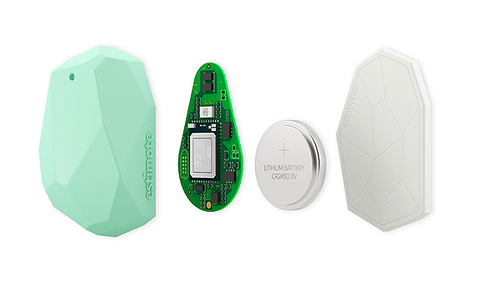
\includegraphics[width=0.7\textwidth]{estimote-beacon}
    \caption{
        \emph{Beacon} da \emph{Estimote} com os componentes: capa de borracha (impermeável), \emph{hardware} com \emph{firmware} e \emph{Bluetooth}, bateria e protetor no fundo
    }
\end{figure}

\subsection{Funcionamento}

O funcionamento do \emph{Beacon}, depende principalmente de três elementos que são configuráveis: o intervalo de disparo de sinal (normalmente em torno de 600ms) e a força do sinal, que é o que irá determinar a distância máxima atingida pelo \emph{Beacon}. O sistema operacional \emph{iOS} faz o scan dos dispositivos a cada 1 segundo, isto significa que se o o \emph{Beacon} estiver com intervalo de disparo em 330ms, o iOS irá receber três vezes o sinal naquele momento. Esta configuração normalmente é feita para lugares mais barulhentos, onde o sinal pode não chegar sempre ao celular, por motivos de outras ondas interferirem na comunicação \cite{beacon-how-it-works-estimote}.

\begin{figure}[h]
\centering
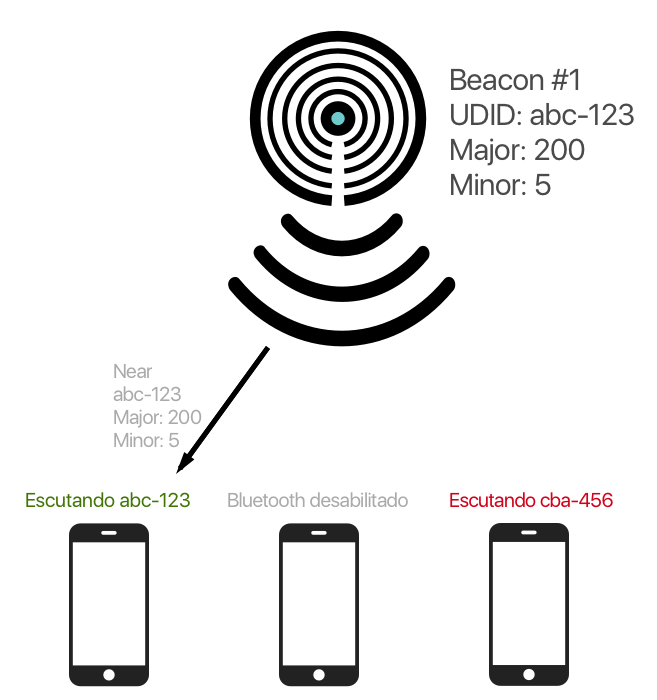
\includegraphics[width=0.85\textwidth]{beacon-how-it-works}
    \caption{
        A imagem mostra o comportamento do \emph{Beacon} com três telefones, um escutando-o, outro com Bluetooth desligado e outro escutando outro \emph{Beacon}. Fonte: Autor.
    }
\end{figure}

\subsection{Segurança}

O \emph{Beacon} é considerada uma tecnologia muito segura, principalmente pelo fato de ela depender da aprovação do usuário para seu funcionamento interferi-lo, pois em primeiro lugar, é necessário que o usuário tenha instalado um aplicativo que consiga ficar escutando as ondas de certos \emph{Beacons}, e mesmo que o usuário tenha o aplicativo instalado, ele ainda precisa aprovar o monitoramento dos \emph{Beacons}, podendo aprovar e restringir a qualquer momento \cite{beacon-what-is-it-forbes}.

\section{Tecnologias}

\subsection{Swift}

Swift é uma linguagem \emph{open-source} extremamente moderna que foi liberada para o público em 2014, mas seu desenvolvimento inicou em 2010. Ela foi desenvolvida pela Apple, mas não é utilizada exclusivamente para seu ecossistema. Conquistou rapidamente os desenvolvedores de aplicativos para iOS e hoje é utilizada na grande maioria dos novos aplicativos.

Como dito em \cite{swift-about}, Swift é uma linguagem estática, compilada e com uma sintaxe muito moderna que traz bastante segurança e rapidez aos desenvolvedores.

\subsection{Web Services}

\emph{Web service} é uma interface que descreve uma coleção de operações que são acessíveis através da internet padronizados em \emph{XML}, \emph{JSON} ou algum tipo de padrão de informações conhecido, desde que todas as operações sigam o mesmo padrão. Ele providência todos os meios para a comunicação da aplicação com o servidor, tornando a comunicação padrão e centralizada para todas as aplicações do serviço \cite{introduction-web-services}.

Para o desenvolvimento dos \emph{web services}, serão utilizadas diversas tecnologias em conjunto, proporcionando assim um sistema facilmente escalável e seguro. Ele utilizará o padrão \emph{JSON} em seus serviços para que as mesmas possam ser utilizadas por todos os softwares que conversarão com a plataforma, seja ele um aplicativo ou um servidor que se integrará, fornecendo ou pedindo informações.

\subsubsection{Infraestrutura}

Na infraestrutura, foi optado a utilização de software livre e de código-aberto, já conhecidos no mercado há muitos anos, por serem mais maduros e por consequência mais seguros e estáveis.

Como servidor \emph{HTTP}, será utilizado o \emph{Nginx}, criado em 2002 com o objetivo de servir sites com um enorme volume de acessos. É um software bastante leve e utilizado mundialmente hoje em aplicações de grande escala \cite{nginx-book}.

O sistema operacional utilizado no servidor será o \emph{Ubuntu Server LTS 16.04}, também é um software livre e de código aberto. Também foi escolhido este sistema operacional pelo fato de os autores já terem conhecimento prévio na utilização da tecnologias nesta plataforma, facilitando o desenvolvimento.

\subsubsection{Django}

Em questões de aplicação no \emph{web service}, será utilizado \emph{Django}, que é um \emph{framework} utilizado em aplicações \emph{Python}, que fornece inúmeras facilidades como: \emph{ORM (Object-relational mapping)}, construção de \emph{API}, migrações de bancos de dados e um painel administrativo que se constrói automaticamente baseado no modelo do banco de dados.

Django utiliza o padrão \emph{MTV (Model-Template-View)} e o princípio \emph{DRY (Don't repeat yourself)} para o desenvolvimento. Isto faz com que exista uma separação muito clara entre o modelo, o template e o design do projeto, tornando-se mais fácil de reutilizar código e testar unitariamente os métodos e classes \cite{django-wikipedia}. 

\subsubsection{JSON}

Toda a comunicação entre a \emph{API} e as aplicações será feita no padrão \emph{JSON (JavaScript Object Notation)}, deixando assim uma comunicação uniforme e utilizando um padrão amplamente conhecido no mundo inteiro, de fácil leitura e compreensão \cite{footnote-json}.



% ----------------------------------------------------------
% Justificativa
% ----------------------------------------------------------

\chapter{Justificativa}

Conforme o gráfico abaixo, pode-se notar que o crescimento do uso de smartphones no Brasil cresce drasticamente a cada ano, deixando claramente evidente que grande parte da população tem, pelo menos, um smartphone.

\begin{figure}[h]
\centering
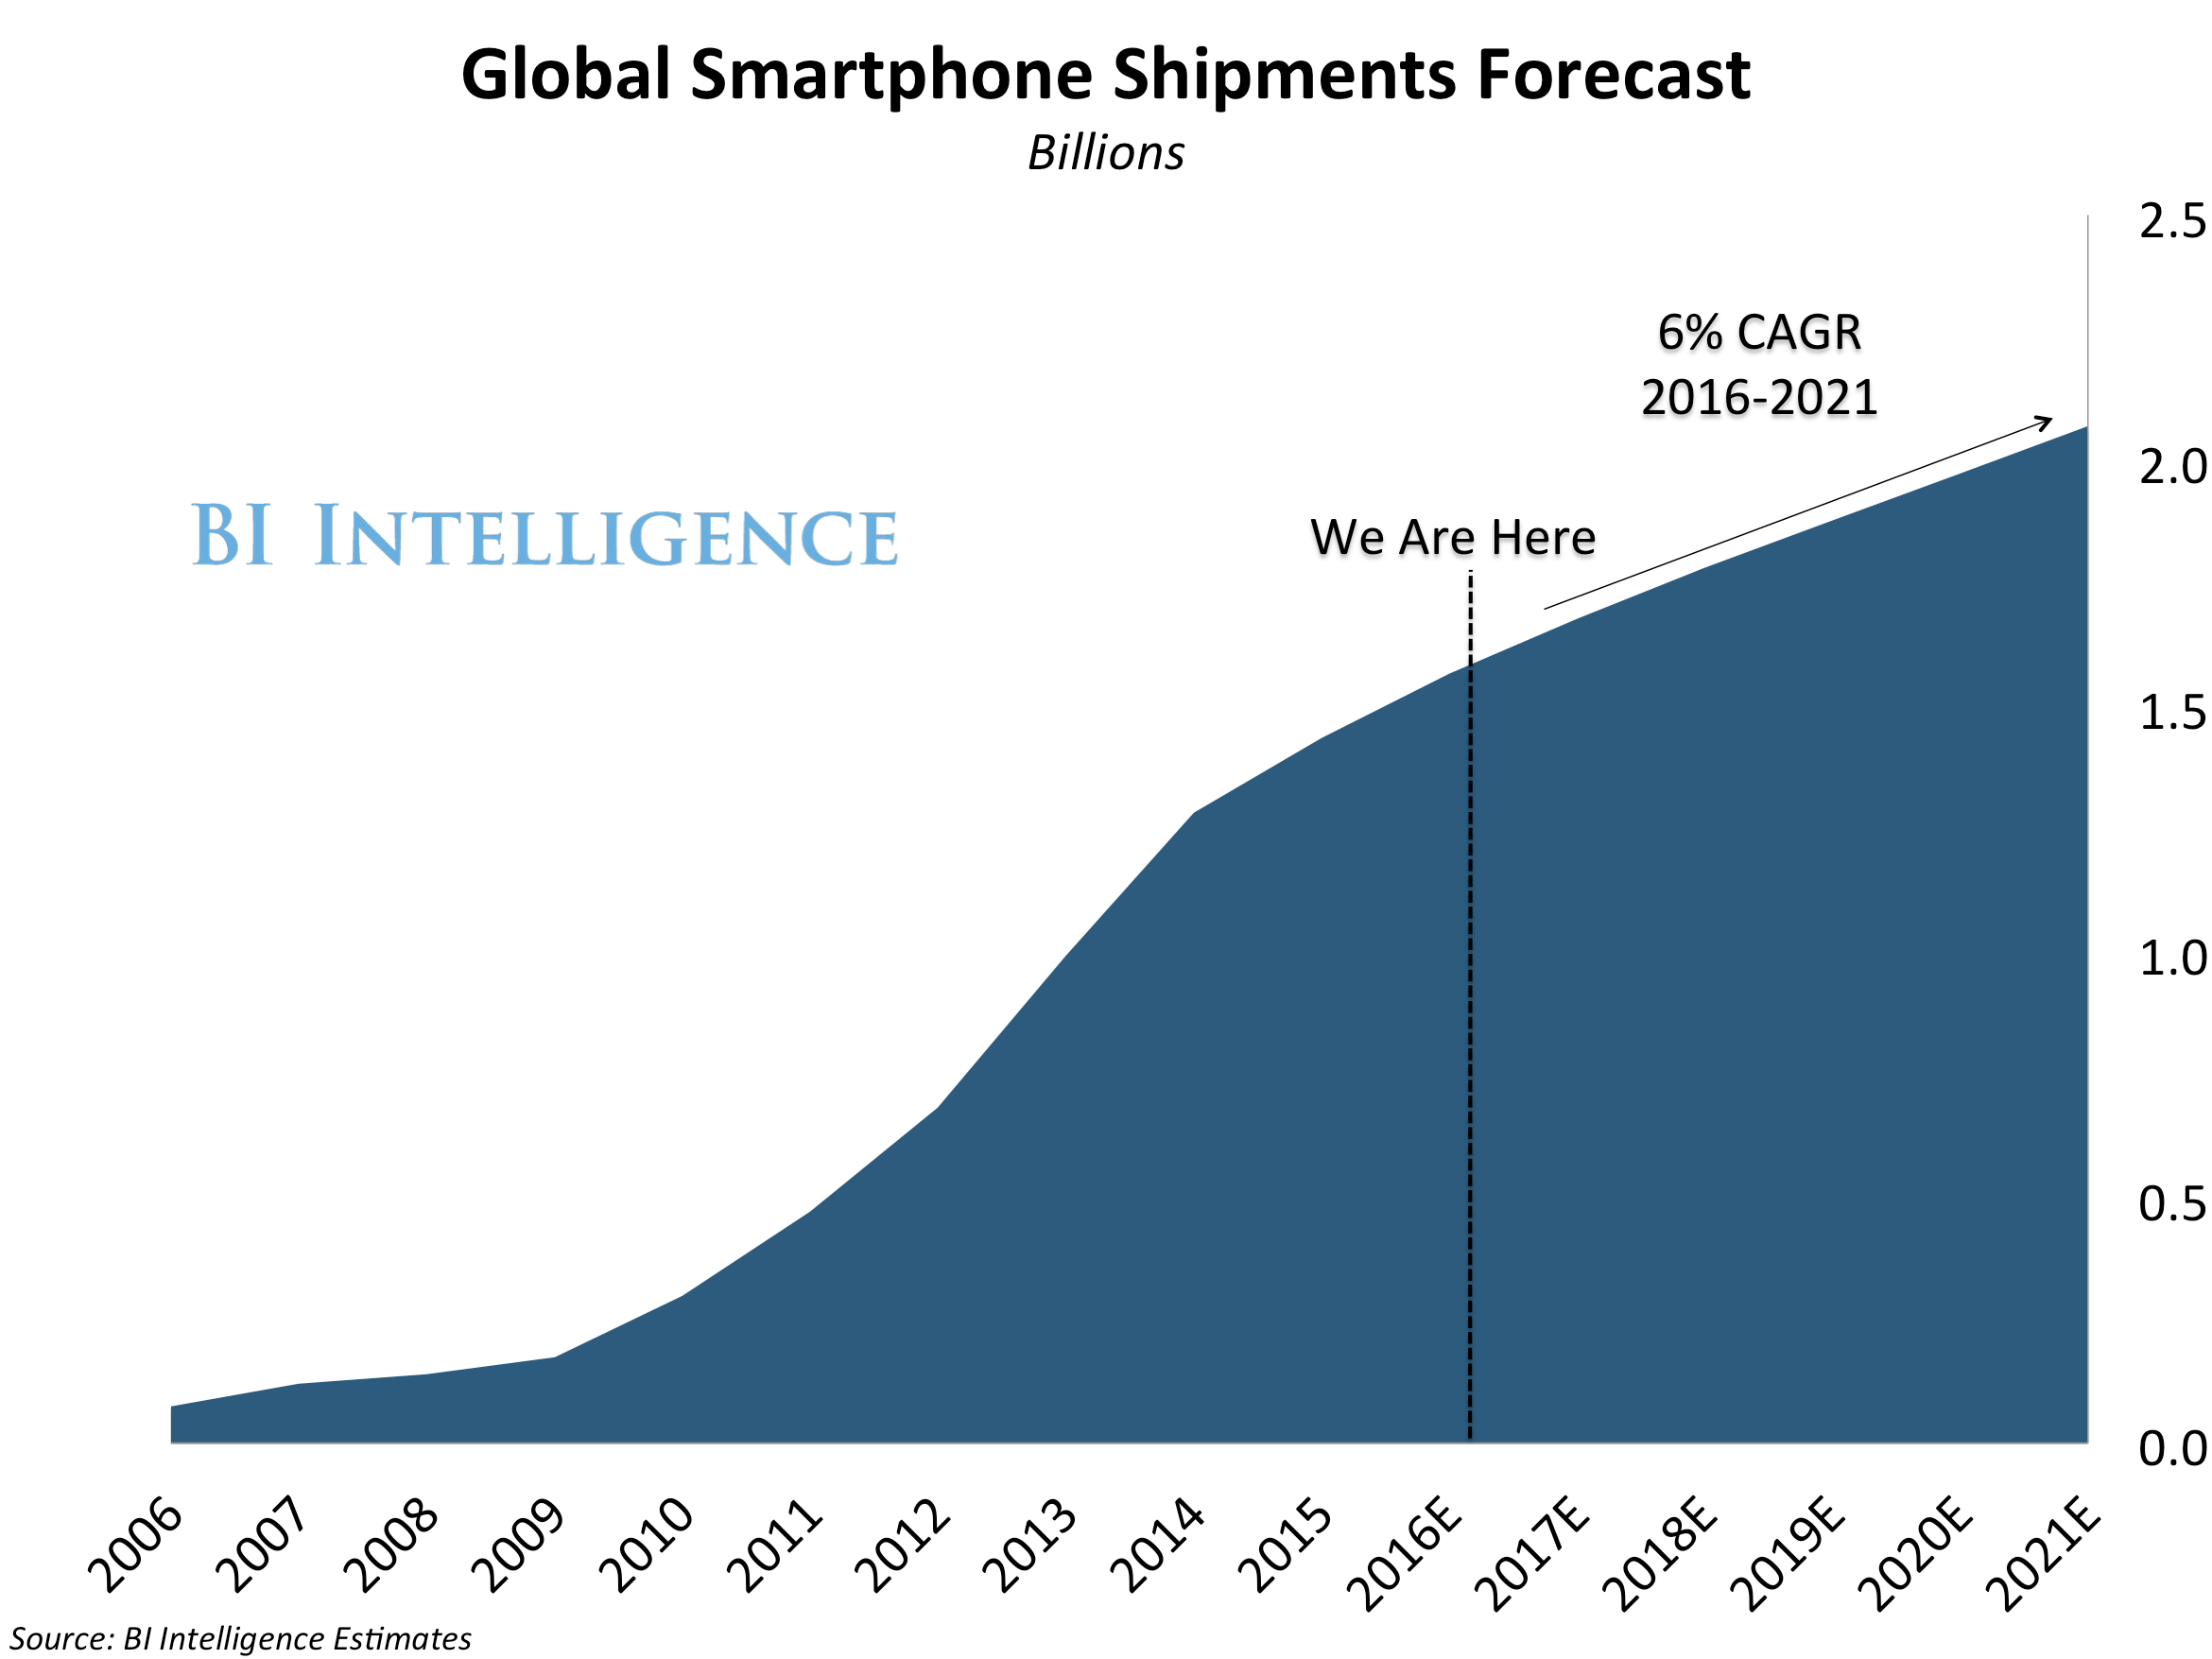
\includegraphics[width=1.0\textwidth]{smartphone_sales}
    \caption{
        Número de vendas de smartphones no mundo e uma projeção para o futuro, até 2021 \cite{smartphone-numbers-image}.
    }
\end{figure}

Com com estas informações, pode-se entender que a maioria das pessoas que frequenta uma instituição de ensino, terá um \emph{smartphone} em mãos. Levando em consideração que a maioria dos \emph{smartphones} no mercado tem a tecnologia \emph{Bluetooth}, pode-se entender então, que é uma tecnologia bastante presente nos dias atuais, tendendo a ser mais presente ainda com a entrada de novos dispositivos que aderirem a tecnologia \cite{bluetooth-devices}.

Neste cenário, diante dos problemas citados no capítulo de problematização, foi concluído que pode-se resolver os problemas utilizando uma tecnologia como o \emph{Bluetooth}, otimizando o tempo gasto em sala de aula, deixando-a mais produtiva e dinâmica.


% ----------------------------------------------------------
% Objetivos
% ----------------------------------------------------------

\chapter{Objetivos}

\section{Objetivos gerais}
Otimizar as atividades de registro de presenças de alunos (controle de frequência em sala de aula) através do desenvolvimento e disponibilização de um produto com a utilização de \emph{Beacons} e \emph{smartphones}.

\section{Objetivos específicos}
\begin{enumerate}
  \item Desenvolver uma aplicação web para fornecimento de informações dos alunos aos aplicativos através de uma \emph{API}, além de fornecer as informações de presença aos professores em formato de relatório;
  \item Desenvolver uma aplicação para \emph{iOS} que será utilizada pelos alunos para a marcação de presença em sala de aula de forma automática, utilizando \emph{Beacons} que serão instalados em salas de aula e na instituição de ensino;
  \item Testar aplicação em uma sala de aula de alguma instituição de ensino com um grupo de alunos, durante pelo menos 3 meses;
\end{enumerate}

% ----------------------------------------------------------
% Resultados Esperados
% ----------------------------------------------------------

\chapter{Resultados esperados}

Espera-se atingir o objetivo proposto, tornando viável um melhor controle de presença dos alunos em instituições de ensino, mais produtivo e mais eficaz do que o atual praticado pela maioria das instituições.
O sucesso desta aplicação, bem como sua comercialização, também é esperada, podendo assim, ser aplicada em diversas instituições de ensino com cenários diferentes.


% ----------------------------------------------------------
% Metodologia
% ----------------------------------------------------------

\chapter{Metodologia}
\section{Proposta do sistema}

Este projeto propõe o desenvolvimento de uma aplicação para \emph{iOS}, que poderá ser publicada na \emph{App Store}\footnote{Loja oficinal de aplicativos para iOS, maiores informações em: https://developer.apple.com/app-store/}, onde alunos das instituições de ensino irão se autenticar para efetivamente usa-lo para que a chamada em sala de aula seja feita de forma automática. Além desta aplicação, também será desenvolvido um servidor web, que poderá ser hospedado em qualquer serviço de \emph{Cloud Computing}\footnote{Computação em Nuvem, onde as preocupações com a largura de banda, espaço de armazenamento, poder de processamento, fiabilidade e segurança, são postas de parte\cite{cloud-computing-about}} (\emph{AWS}\footnote{https://aws.amazon.com/pt/}, por exemplo). Neste servidor estará toda a integração com o aplicativo para \emph{iOS} e demais plataformas futuramente, como \emph{Android}\footnote{Sistema Operacional Open Source desenvolvido pelo Google e disponível em: https://android.com/intl/pt\-BR\_br/}, por exemplo.

\subsection{Aplicativo iOS}

O aplicativo iOS é a aplicação na qual o aluno irá interagir, autenticando-se e vendo informações de suas disciplinas matriculadas, além de permitir acesso Bluetooth e de localização ao aplicativo, para que a presença do aluno seja marcada automaticamente nas disciplinas, através dos \emph{Beacons} instalados em sala de aula.

O aluno, após autenticar-se, poderá acompanhar quais cadeiras está matriculado em uma listagem e dentro de cada cadeira poderá ver informações importantes como: nome do professor, e-mail do professor, sala de aula, data da próxima aula, quantidade de presenças e faltas e se possível, as notas da cadeira.

\subsection{Servidor Web}

O servidor web servirá como um apoio fundamental para o funcionamento do aplicativo, pois nele estarão todos os dados sincronizados entre o software e a instituição de ensino, além das informações providas do próprio aluno automaticamente, através dos \emph{Beacons}.

Além de armazenar os dados, ele terá uma \emph{API}\footnote{Application Programming Interface: interface padrão para comunicação entre os dispositivos \cite{footnote-api}.} que fornecerá as informações no formato \emph{JSON}\footnote{Padrão aberto de comunicação em formato de objeto JavaScript, de fácil leitura e compreensão \cite{footnote-json}.} para as aplicações (e demais futuras que queiram integrar). Toda a comunicação com o servidor é feita de forma segura, utilizando o protocolo \emph{SSL}\footnote{Secure Sockets Layer: protocolo seguro de comunicação, que criptografa as informações através de um certificado seguro e validado \cite{footnote-ssl}}. 

\section{Desenvolvimento do sistema}
\subsection{Análise}

Será feito uma análise de quais os elementos (e suas características) existentes em um ambiente de chamadas de uma instituição de ensino superior que podem ajudar na elaboração do projeto, com informações importantes e até mesmo obrigatórias, do ponto de vista jurídico.

\subsection{Projeto}

A partir dos dados analisados, serão criados diagramas que demonstrarão a estrutura e fluxo da aplicação. Em seguirá será feito o projeto da interface com \emph{mockups} do aplicativo para visualização.

\subsection{Codificação}

A codificação deste produto será utilizando o paradigma de orientação à objetos. As linguagens serão \emph{Swift} e \emph{Python}. Para que esta aplicação possa ser desenvolvida, será utilizado a \emph{IDE} \emph{Xcode} para criação do aplicativo \emph{iOS} e um editor de textos para a criação da aplicação web. Para realizar os testes e também utilizar a aplicação, será necessário pelo menos um dispositivo com \emph{iOS}, um navegador web e um \emph{Beacon}.

\subsection{Testes}

Tanto a aplicação web quanto a aplicação para \emph{iOS} terão testes unitários automatizados, além dos testes que serão realizados manualmente para a identificação da posição e potência de sinal do \emph{Beacon}, para encontrar assim o melhor cenário em uma sala de aula para seu funcionamento. Após o término do desenvolvimento inicial da aplicação, pretende-se testar com alguns alunos em uma sala de aula por pelo menos 3 meses, para assim certificar-se de que o sistema está realmente oferecendo o suporte necessário.

\subsection{Implantação}

O \emph{software} a ser desenvolvido será instalado em um servidor na nuvem \emph{Ubuntu Server LTS} e a aplicação \emph{iOS} inicialmente será distribuída através do \emph{TestFlight}, que é uma plataforma de distribuição fornecida para a \emph{Apple} enquanto a aplicação não está disponível para o público. Quando a aplicação estiver pronta para o público, ela será publicada na \emph{App Store}, sendo assim, acessível por todos.

\section{Manutenção do sistema}

O software utilizará \emph{git}\footnote{Sistema de controle de versão amplamente utilizado no mundo, disponível em: https://git-scm.com} para controle de versão, na plataforma do \emph{GitHub} de forma privada. Nunca sendo alterado código diretamente em produção ou qualquer outro meio que não esteja vinculado ao controle de versão.

Também haverá marcação de \emph{tags} para cada versão oficial enviada, tanto nos aplicativos móveis quanto no código do servidor.

\section{Tecnologias e ferramentas}

O desenvolvimento do software para \emph{iOS} será desenvolvimento na \emph{IDE} \footnote{Integrated Development Enviroment}, ou Ambiente Integrado para desenvolvimento) \emph{Xcode}, fornecido pela Apple para desenvolvimento de aplicativos \emph{iOS} e \emph{macOS}.

Na aplicação web, serão utilizadas ferramentas já muito maduras no mercado, com o objetivo de ter uma aplicação estável, de fácil manutenção e segura. A primeira camada de comunicação do servidor será feita com \emph{Nginx}\footnote{Servidor Web mundialmente conhecido e utilizado, disponível em: https://nginx.com}, seguida do \emph{Gunicorn}\footnote{Servidor Python WSGI HTTP para Linux, disponível em: http://gunicorn.org}, responsável por manter a aplicação feita em \emph{Django}\footnote{Framework Python amplamente utilizado, disponível em: https://djangoproject.com} sempre ligada, respondendo as demandas dos usuários. O \emph{Django} oferece soluções muito fáceis e eficientes para a construção de um banco de dados, que neste caso será o \emph{PostgreSQL}\footnote{Banco de Dados Open Source, disponível em: https://postgresql.org}, para a construção de um painel administrativo e também de um API.


% ----------------------------------------------------------
% Orçamento  
% ----------------------------------------------------------

\chapter{Orçamento}

\noindent
\begin{table}[ht]
    \caption{Investimento Inicial Fixo}
    
    \begin{tabularx}{\textwidth}{X|c|r|r}
    \hline
        \textbf{Descrição} &
        \textbf{Quantidade} & 
        \textbf{Valor unitário} & 
        \textbf{Valor total} \\
    \hline
        Apple MBPr 15" 16GB 500GB SSD&1&R\$18.000&R\$18.000 \\
        iPhone 7 128GB&2&R\$4.000&R\$8.000 \\
        Beacon Estimote&10&R\$120&R\$1.200 \\ [1ex]
    \hline
        \textbf{Total}&&&\textbf{R\$27.000} \\ [1ex]
    \end{tabularx}
\end{table}

\noindent
\begin{table}[ht]
    \caption{Investimento com pessoas}

    \begin{tabularx}{\textwidth}{X|l|c|r|r}
    \hline
        \textbf{Nome} & 
        \textbf{Função} & 
        \textbf{Quantidade} & 
        \textbf{Valor hora} &
        \textbf{Valor total} \\
    \hline
        Rafael K. Streit&Desenvolvedor &300&R\$100&R\$30.000\\
        Eurico Antunes&Orientador&60&R\$200&R\$12.000 \\
    \hline
        \textbf{Total} &&&& \textbf{R\$32.000} \\
    \end{tabularx}
\end{table}

\noindent
\begin{table}[ht]
    \caption{Investimento Mensal}
    \begin{tabularx}{\textwidth}{X|c|r}
    \hline
        \textbf{Descrição} &
        \textbf{Quantidade} &
        \textbf{Valor} \\
    \hline
        Servidor Ubuntu Server na AWS &1 &R\$100 \\
    \hline
        \textbf{Total}&&\textbf{R\$100} \\ [1ex]
    \end{tabularx}
\end{table}


% ----------------------------------------------------------
% Cronograma  
% ----------------------------------------------------------

\chapter{Cronograma}

\begin{figure}[h]
\centering
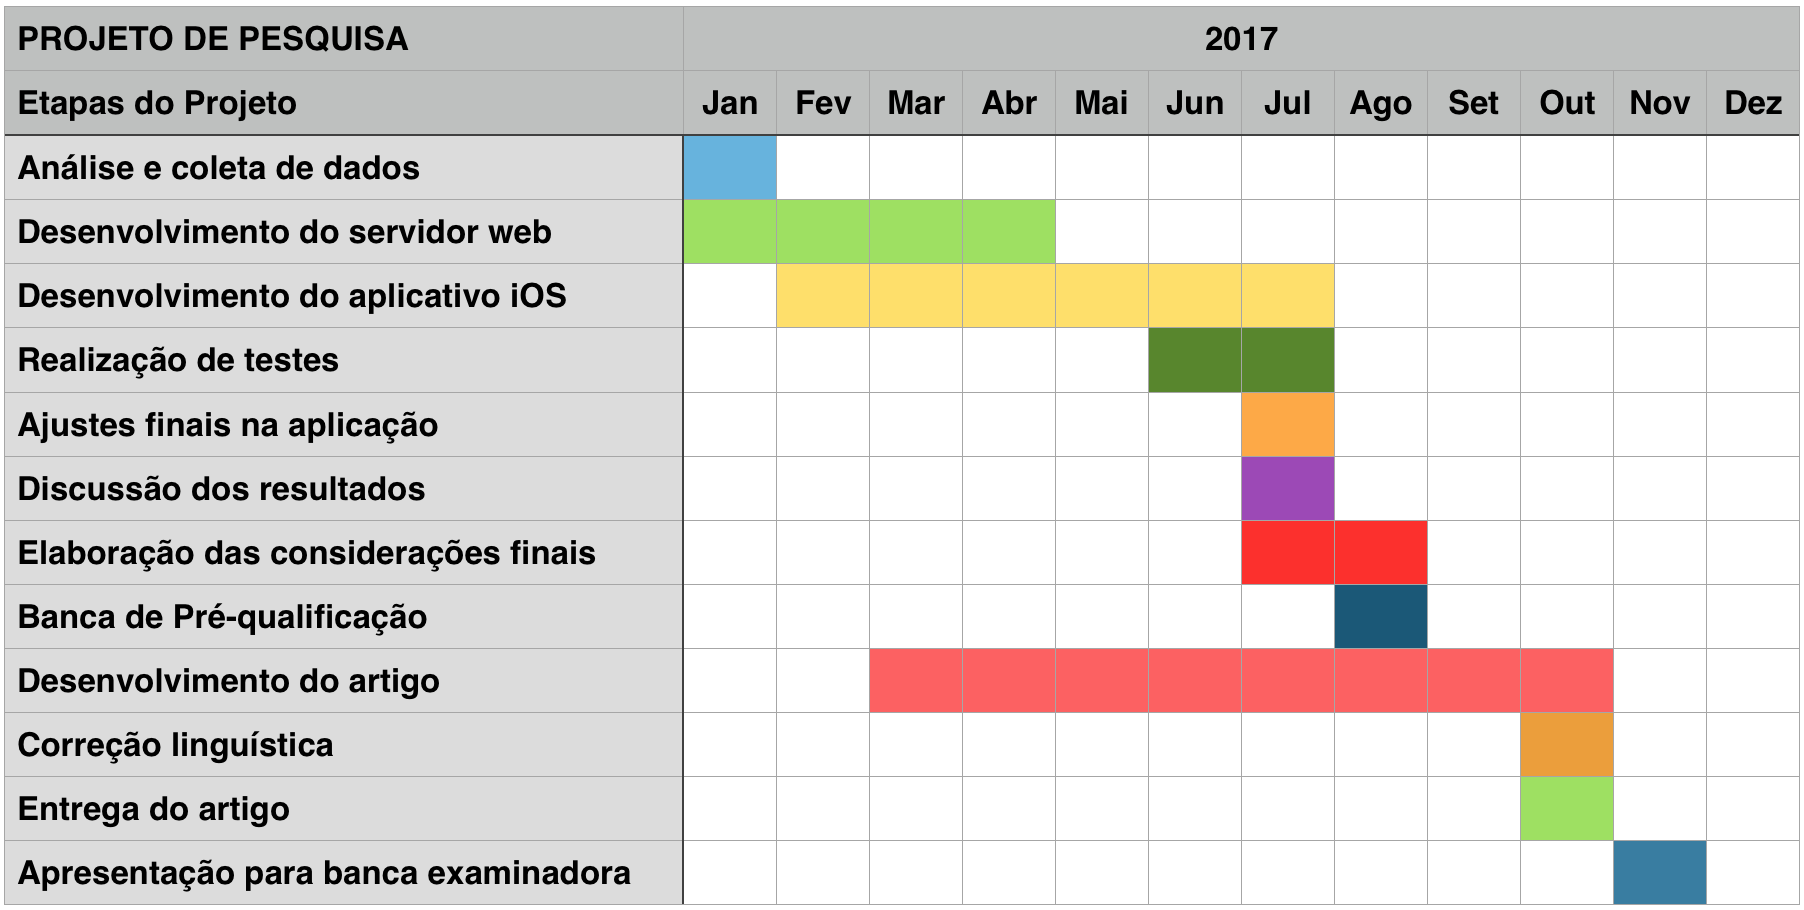
\includegraphics[width=1.0\textwidth]{cronograma}
\end{figure}


% ----------------------------------------------------------
% ELEMENTOS PÓS-TEXTUAIS
% ----------------------------------------------------------
\postextual

% ----------------------------------------------------------
% Referências bibliográficas
% ----------------------------------------------------------
\bibliography{Referencias}

% ----------------------------------------------------------
% Glossário
% ----------------------------------------------------------
%
% Consulte o manual da classe abntex2 para orientações sobre o glossário.
%
%\glossary

\end{document}
